% =====================================================================
% NOTE DE RECHERCHE — Calibrage et simulation du GSE IRCANTEC
% Représentation autorégressive agrégée à régime latent commun :
% estimation par maximum de vraisemblance jointe et simulation cohérente.
% Cadre GENERAL : aucune corrélation fixée a priori ; toute la dépendance
% est estimée librement, par régime, sur les résidus standardisés.
% Charte Nexialog v2 (mai 2026). Polices Montserrat + Source Sans Pro
% avec repli automatique (Times + Helvetica) si non installées.
% Compilation : pdflatex (x2). Document autonome (logo en repli texte).
% =====================================================================
\documentclass[11pt,a4paper]{article}

% --------- PACKAGES ---------------------------------------------------
\usepackage[utf8]{inputenc}
\usepackage[T1]{fontenc}
\IfFileExists{sourcesanspro.sty}{\usepackage[default]{sourcesanspro}}{\usepackage{mathptmx}}
\IfFileExists{montserrat.sty}{\usepackage{montserrat}}{\usepackage[scaled=0.92]{helvet}}
\usepackage{microtype}
\usepackage{cmap}
\usepackage{geometry}
\usepackage{graphicx}
\usepackage{xcolor}
\usepackage{amsmath,amssymb,amsthm,mathtools,bm}
\usepackage{textcomp}
\usepackage{fancyhdr}
\usepackage{titlesec}
\usepackage[hyperref]{etoc}
\usepackage{enumitem}
\usepackage{tcolorbox}
\usepackage{xurl}
\usepackage{hyperref}
\usepackage{booktabs}
\usepackage{colortbl}
\usepackage{array}
\usepackage{longtable}
\usepackage{float}
\usepackage{caption}
\usepackage{tabularx}
\usepackage{tikz}
\usetikzlibrary{arrows.meta,positioning,calc,fit,backgrounds}
\usepackage{needspace}
\usepackage{etoolbox}

% --------- CHARTE NEXIALOG (officielle v2) ----------------------------
\definecolor{nxnavy}{HTML}{002060}
\definecolor{nxred}{HTML}{B10031}
\definecolor{nxteal}{HTML}{409ABB}
\definecolor{nxslate}{HTML}{223E55}
\definecolor{nxgray}{HTML}{9A999E}
\definecolor{nxlightgray}{HTML}{D0D1D4}
\definecolor{nxoffwhite}{HTML}{F2F2F2}
\definecolor{nxgreen}{HTML}{2E7D32}
\definecolor{nxorange}{HTML}{F57C00}
\definecolor{nxlightblue}{HTML}{E6ECF7}

% --------- LOGO (repli texte si le PDF est absent) -------------------
\newcommand{\nxlogo}[1][0.50\textwidth]{%
  \IfFileExists{logo_nexialog.pdf}%
    {\includegraphics[width=#1]{logo_nexialog.pdf}}%
    {\parbox{#1}{\centering\sffamily\bfseries\color{nxnavy}\fontsize{30}{34}\selectfont NEXIALOG\\[1mm]{\normalsize\color{nxred}\,CONSULTING}}}}
\newcommand{\nxlogosmall}{%
  \IfFileExists{logo_nexialog.pdf}%
    {\includegraphics[height=13mm]{logo_nexialog.pdf}}%
    {\sffamily\bfseries\color{nxnavy}\large NEXIALOG\,{\color{nxred}\small C.}}}

% --------- PAGE SETUP -------------------------------------------------
\geometry{a4paper, top=32mm, bottom=22mm, left=25mm, right=25mm,
          headheight=19mm, headsep=6mm}

% --------- HEADER / FOOTER --------------------------------------------
\pagestyle{fancy}
\fancyhf{}
\fancyhead[L]{\parbox[c][14mm][c]{52mm}{\nxlogosmall}}
\fancyhead[R]{\parbox[c][14mm][c]{110mm}{\raggedleft\small GSE IRCANTEC~~\textbar~~\textit{Note de recherche --- Calibrage \& simulation}}}
\fancyfoot[L]{\small Note de recherche --- Juin 2026}
\fancyfoot[R]{\small Page \thepage}
\renewcommand{\headrulewidth}{0pt}
\renewcommand{\footrulewidth}{0.3pt}
\renewcommand{\footrule}{\hbox to\headwidth{\color{nxlightgray}\leaders\hrule height \footrulewidth\hfill}}

% --------- STYLES DE SECTION (Montserrat) -----------------------------
\titleformat{\section}{\sffamily\Large\bfseries\color{nxnavy}}{\thesection.}{0.5em}{}
\titleformat{\subsection}{\sffamily\large\bfseries\color{nxnavy}}{}{0em}{\thesubsection.~}
\titleformat{\subsubsection}{\sffamily\normalsize\bfseries\color{nxnavy}}{}{0em}{\thesubsubsection.~}

% --------- TABLE DES MATIÈRES (etoc) ----------------------------------
\etocsetstyle{section}{}{}
  {\par\noindent\sffamily\large\bfseries\textcolor{nxred}{\etocname}\hfill\textcolor{nxred}{\etocpage}\par\medskip}{}
\etocsetstyle{subsection}{}{}
  {\par\noindent\hspace*{5mm}\sffamily\normalsize\mdseries\textcolor{nxnavy}{\etocname}\hfill\textcolor{nxnavy}{\etocpage}\par\vspace{6pt}}{}
\etocsetstyle{subsubsection}{}{}
  {\par\noindent\hspace*{10mm}\sffamily\small\mdseries\textcolor{nxnavy}{\etocname}\hfill\textcolor{nxnavy}{\etocpage}\par\vspace{5pt}}{}
\etocsettocstyle{}{}

% --------- ENVIRONNEMENTS PERSONNALISÉS -------------------------------
\tcbuselibrary{skins,breakable}
\newtcolorbox{definitionbox}[1][]{enhanced, breakable,
  colback=nxlightblue, frame hidden, boxrule=0pt, arc=3pt,
  before skip=4mm, after skip=3mm, left=4mm, right=4mm, top=3mm, bottom=3mm}

\newtcolorbox{insightbox}[1][Point clé]{enhanced, breakable,
  colback=nxoffwhite, frame hidden, boxrule=0pt, arc=3pt,
  fonttitle=\sffamily\bfseries\color{nxred}, title={#1},
  detach title, before upper={\tcbtitle\par\nobreak\medskip\nobreak},
  before skip=4mm, after skip=3mm, left=4mm, right=4mm, top=3mm, bottom=3mm}

\newtcolorbox{mabox}[1][]{enhanced, breakable,
  colback=nxlightblue, frame hidden, boxrule=0pt, arc=3pt,
  fonttitle=\sffamily\bfseries\color{nxnavy}, title={#1},
  detach title, before upper={\tcbtitle\par\nobreak\medskip\nobreak},
  before skip=4mm, after skip=3mm, left=4mm, right=4mm, top=3mm, bottom=3mm}

\newtcolorbox{algobox}[1][Algorithme]{enhanced, breakable,
  colback=white, colframe=nxnavy, boxrule=0.8pt, arc=3pt,
  fonttitle=\sffamily\bfseries\color{white}, coltitle=white,
  colbacktitle=nxnavy, title={#1},
  before skip=4mm, after skip=3mm, left=4mm, right=4mm, top=3mm, bottom=3mm}

\theoremstyle{definition}
\newtheorem{proposition}{Proposition}
\newtheorem{remarque}{Remarque}

% --------- CAPTIONS / FLOATS ------------------------------------------
\captionsetup{font=small,labelfont={bf,color=nxnavy},labelsep=period}
\setlength{\abovecaptionskip}{4pt}\setlength{\belowcaptionskip}{4pt}
\setlength{\textfloatsep}{10pt plus 2pt minus 2pt}
\setlength{\floatsep}{8pt plus 2pt minus 2pt}
\setlength{\intextsep}{10pt plus 2pt minus 2pt}
\renewcommand{\topfraction}{0.92}\renewcommand{\bottomfraction}{0.92}
\renewcommand{\textfraction}{0.05}\renewcommand{\floatpagefraction}{0.85}
\widowpenalty=10000\clubpenalty=10000

% --------- LISTES & ANTI-ORPHELINS ------------------------------------
\setlist{leftmargin=*, labelindent=0pt, itemsep=2pt, topsep=4pt}
\pretocmd{\section}{\needspace{6\baselineskip}}{}{}
\pretocmd{\subsection}{\needspace{5\baselineskip}}{}{}
\pretocmd{\subsubsection}{\needspace{4\baselineskip}}{}{}
\BeforeBeginEnvironment{definitionbox}{\needspace{5\baselineskip}}
\BeforeBeginEnvironment{insightbox}{\needspace{5\baselineskip}}
\BeforeBeginEnvironment{mabox}{\needspace{4\baselineskip}}
\BeforeBeginEnvironment{algobox}{\needspace{6\baselineskip}}

% --------- HYPERREF ---------------------------------------------------
\hypersetup{colorlinks=true, linkcolor=nxred, citecolor=nxred, urlcolor=nxred,
  linktoc=all, pdftitle={Note de recherche -- Calibrage et simulation du GSE IRCANTEC},
  pdfauthor={Nexialog Consulting}}

% --------- OPÉRATEURS / RACCOURCIS MATH -------------------------------
\DeclareMathOperator{\Corr}{Corr}
\DeclareMathOperator{\Var}{Var}
\DeclareMathOperator{\Cov}{Cov}
\DeclareMathOperator{\diag}{diag}
\DeclareMathOperator{\tr}{tr}
\DeclareMathOperator{\chol}{chol}
\DeclareMathOperator{\vecop}{vec}
\DeclareMathOperator*{\argmin}{arg\,min}
\DeclareMathOperator*{\argmax}{arg\,max}
\newcommand{\R}{\mathbb{R}}
\newcommand{\E}{\mathbb{E}}
\newcommand{\Prob}{\mathbb{P}}
\newcommand{\Ecal}{\mathcal{E}}
\newcommand{\Ncal}{\mathcal{N}}
\newcommand{\Xcal}{\mathcal{X}}
\newcommand{\eps}{\varepsilon}
\newcommand{\transp}{^{\!\top}}
\newcommand{\dd}{\mathrm{d}}
\newcommand{\Dt}{\Delta}

\setlength{\emergencystretch}{2.5em}
\tolerance=1200

% =====================================================================
\begin{document}
% =====================================================================

% --------- PAGE DE GARDE ----------------------------------------------
\begin{titlepage}
\thispagestyle{empty}
\vspace*{-5mm}
\begin{center}\nxlogo[0.55\textwidth]\end{center}
\vspace{1.4cm}
\begin{center}
  {\color{nxred}\rule{0.6\textwidth}{1.5pt}}\\[10mm]
  {\sffamily\bfseries\color{nxnavy}\fontsize{24pt}{30pt}\selectfont
   \MakeUppercase{Calibrage et simulation du GSE}\\[4mm]
   \MakeUppercase{Représentation autorégressive}\\[2mm]
   \MakeUppercase{à régime latent commun}}\\[10mm]
  {\color{nxred}\rule{0.6\textwidth}{1.5pt}}\\[10mm]
  {\sffamily\large\color{nxnavy}Note de recherche méthodologique}\\[3mm]
  {\sffamily\normalsize\color{nxnavy}Juin 2026}
\end{center}
\vspace{10mm}
\noindent\begin{minipage}{\textwidth}\small
Cette note de recherche est un document \textbf{autonome} consacré à l'\emph{estimation} et à la \emph{simulation} du générateur de scénarios économiques (GSE) monde réel du régime IRCANTEC. Elle ne reprend ni le diagnostic critique, ni les volets \emph{courbe des taux}, \emph{pricing} zéro-coupon, prime de liquidité ou \emph{smoothing} : on s'y limite, pour chaque facteur de risque, au \emph{modèle de diffusion} et à sa \emph{discrétisation} (exacte ou approchée, au pas $\Dt$), puis on construit un \textbf{unique modèle autorégressif agrégé} à régime latent commun regroupant tous les facteurs.

\vspace{2mm}
Le cadre est \textbf{général} : aucune corrélation n'est fixée \emph{a priori} (ni à zéro, ni à dire d'expert). Toute la dépendance --- entre facteurs, à l'intérieur d'un facteur vectoriel, et selon le régime --- est \emph{estimée librement} sur les résidus standardisés. L'objet central est la \textbf{méthodologie de calibrage par maximum de vraisemblance jointe} (et non par appariement de moments ni régression \emph{ad hoc}), déclinée en une procédure séquentielle en trois étapes --- marges, régime commun, corrélations par régime --- avec \emph{formes fermées explicites} partout où elles existent, puis la \textbf{technique de simulation} cohérente associée. Le dernier chapitre applique le cadre à un AR regroupant l'intégralité des facteurs et en donne toutes les \emph{expressions littérales finales}, directement implémentables. Document confidentiel, à usage méthodologique exclusif de l'IRCANTEC et de la Caisse des Dépôts.
\end{minipage}
\vfill
\begin{center}{\sffamily\bfseries\large\color{nxnavy}THINK SMART~~\textcolor{nxred}{$\bullet$}~~ACT DIFFERENT}\end{center}
\end{titlepage}

% --------- TABLE DES MATIÈRES -----------------------------------------
\begingroup
\hypersetup{hidelinks}
\vspace*{\stretch{0.5}}
{\noindent\sffamily\Huge\bfseries\color{nxnavy}Table des matières\par}
\vspace{16mm}
\tableofcontents
\vspace*{\stretch{2}}
\endgroup
\newpage

% =====================================================================
\section{Objet et périmètre}

Le GSE du régime simule par Monte-Carlo, sur un horizon ALM long ($\sim30$~ans), l'ensemble des facteurs de risque alimentant l'allocation stratégique. Chaque facteur est diffusé par une EDS propre, discrétisée puis simulée au pas mensuel. Cette note traite deux maillons~: (i)~la \textbf{mise sous forme autorégressive unique} de tous les facteurs, et (ii)~leur \textbf{calibrage} puis leur \textbf{simulation cohérente}.

\begin{insightbox}[Fil directeur]
Toute EDS du GSE, discrétisée, s'écrit comme une \emph{récurrence autorégressive vectorielle} dont les coefficients peuvent dépendre du temps, du pas $\Dt$ et d'un \emph{régime de marché commun} $\Ecal_t$. On agrège tous les facteurs en un \emph{unique} modèle à changement de régime (MS-VAR), on le calibre \emph{par marge puis par dépendance} (procédure séquentielle IFM), et on le simule directement à partir de cette représentation. Estimation et simulation partagent \emph{une seule loi}~; \emph{aucune corrélation n'est imposée}~: toute la dépendance est estimée.
\end{insightbox}

\noindent\textbf{Périmètre.} On rappelle, pour chaque facteur, \emph{uniquement} son modèle de diffusion et sa discrétisation. Le \emph{pricing} de la courbe nominale, les corrections de covariance zéro-coupon, la prime de liquidité et le \emph{déslissage} (\emph{unsmoothing}) ne sont pas traités~: on travaille sur les séries de facteurs qui en résultent.

\noindent\textbf{Parcimonie en hypothèses.} On ne retient que la structure \emph{de diffusion} (dérive, retour à la moyenne, positivité, régime). On n'impose \emph{aucune} contrainte sur les (co)variances de bruit ni sur les corrélations~: la matrice de dépendance est pleinement libre et estimée par régime --- y compris la corrélation interne d'un facteur vectoriel.

% =====================================================================
\section{Notations et conventions}
\label{sec:notations}
% =====================================================================
\noindent\emph{Glossaire de toutes les quantités utilisées dans la note.}
\begin{itemize}[itemsep=2pt]
\item \textbf{Temps, indices, dimensions.} $\Dt=1/12$ (pas mensuel), $n\approx240$ observations (20~ans)~; facteur $i$~; régimes $a,b\in\{1,\dots,K\}$~; $d=\sum_i d_i$ dimension de l'état global (ici $d=12$)~; $D$ nombre d'actifs portant le régime ($D=3$ actions).
\item \textbf{Régime commun $\Ecal_t\in\{1,\dots,K\}$.} Chaîne de Markov de matrice de transition $P=(p_{ab})$, $p_{ab}=\Prob(\Ecal_{t+\Dt}=b\mid\Ecal_t=a)$~; loi invariante $\pi$ ($\pi\transp P=\pi\transp$, probabilités stationnaires)~; $\xi_{t\mid t}(a)$ proba \emph{filtrée} d'être en régime $a$ (vu le passé), $\hat\xi_t(a)$ proba \emph{lissée} (vu tout l'échantillon), $\hat\xi_t(a,b)$ transition lissée (\S\ref{sec:calib}).
\item \textbf{État et innovations.} $Y_t\in\R^d$ état global, $Y^{(i)}_t\in\R^{d_i}$ facteur $i$ ($d_i=2$ pour le V2F, $1$ sinon)~; $\eps_{t+\Dt}\in\R^d$ innovations \emph{standardisées} (marginalement $\Ncal(0,1)$), de matrice de corrélation $\Omega(\Ecal_t)$ \emph{propre au régime}~; $\eps=L(\Ecal_t)z$, $z\sim\Ncal(0,I_d)$, $L(a)$ facteur de Cholesky de $\Omega(a)$.
\item \textbf{Coefficients de la récurrence AR (par facteur).} $\Phi_i$ matrice autorégressive (persistance), $c_i$ constante (niveau), $D_i$ échelle du bruit. Pour le V2F~: $\Phi=e^{-A\Dt}$, $\phi_{12}$ couplage court$\leftarrow$long, $\Sigma_{\mathrm{cond}}=\bigl(\begin{smallmatrix}V_r&C_{mr}\\C_{mr}&V_m\end{smallmatrix}\bigr)$ covariance conditionnelle ($V_r,V_m$ variances, $C_{mr}$ covariance), $\rho_c=C_{mr}/\sqrt{V_rV_m}$ corrélation conditionnelle.
\item \textbf{Paramètres de marge.} \emph{V2F}~: $\kappa_1,\kappa_2$ vitesses de retour à la moyenne (court/long), $\sigma_1,\sigma_2$ volatilités, $\rho$ corrélation des browniens, $\mu$ cible long terme. \emph{CIR}~: $\kappa,\theta,\sigma$ (vitesse, cible, vol)~; $c_\chi,\nu,\lambda$ paramètres d'échelle/degrés/non-centralité du $\chi^2$ décentré. \emph{BK}~: $k,\theta,\sigma$. \emph{Hardy/BS}~: $\mu_a,\sigma_a$ drift/vol (par régime pour Hardy)~; moments par pas $m_a=(\mu_a-\tfrac{\sigma_a^2}{2})\Dt$, $v_a=\sigma_a^2\Dt$.
\item \textbf{Lois et estimation.} $f_i$ densité de transition exacte du facteur $i$, $F_i$ sa f.d.r.~; $\Phi,\varphi$ f.d.r./densité $\Ncal(0,1)$, $\varphi_p(\cdot;m,V)$ densité $\Ncal(m,V)$, $F_{\chi'^2}(\cdot;\nu,\lambda)$ f.d.r.\ du $\chi^2$ décentré~; $\hat\theta$ paramètres estimés, $\ell$ log-vraisemblance, $p_K$ nombre de paramètres libres (pour le BIC).
\item \textbf{Dépendance.} $\widehat\eps_t$ résidu PIT \emph{complet} (tous facteurs empilés)~; $G^{\mathrm{reg}}(a)$ corrélation des résidus dans le régime $a$, $G^{\mathrm{pool}}$ corrélation poolée (tous régimes)~; $S$ masque (corrélations propres au régime ou communes)~; $\delta_a$ intensité de rétrécissement, $n^{\mathrm{eff}}_a$ taille d'échantillon effective du régime~; $\Omega^{\mathrm{SDP}}(a)$ corrélation finale, définie-positive.
\end{itemize}

% =====================================================================
\section{Facteurs : modèle de diffusion et discrétisation}
\label{sec:facteurs}
% =====================================================================
Facteur par facteur~: l'EDS et sa discrétisation au pas $\Dt$ (\emph{exacte} sauf mention). Aucune restriction sur les corrélations.

\subsection{Taux (inflation, taux réels) --- Vasicek à deux facteurs (V2F)}
\label{sec:v2f}
\begin{definitionbox}
\textbf{Modèle.} Un facteur court $q^s_t$ revient vers un facteur long stochastique $q^l_t$, lui-même en retour à la moyenne vers la cible long terme $\mu$~:
\[
\dd q^s_t=\kappa_1(q^l_t-q^s_t)\dd t+\sigma_1\dd W^1_t,\qquad
\dd q^l_t=\kappa_2(\mu-q^l_t)\dd t+\sigma_2\dd W^2_t,\quad \dd\langle W^1,W^2\rangle=\rho\,\dd t .
\]
Avec $X_t=(q^s_t,q^l_t)\transp$, $A=\bigl(\begin{smallmatrix}\kappa_1&-\kappa_1\\0&\kappa_2\end{smallmatrix}\bigr)$, $\Sigma_w=\bigl(\begin{smallmatrix}\sigma_1^2&\rho\sigma_1\sigma_2\\\rho\sigma_1\sigma_2&\sigma_2^2\end{smallmatrix}\bigr)$~: $\dd X_t=A(\mu_\infty-X_t)\dd t+\Sigma_w^{1/2}\dd W_t$, $\mu_\infty=(\mu,\mu)\transp$.

\smallskip\textbf{Discrétisation exacte.} $X_{t+\Dt}=\Phi X_t+(I-\Phi)\mu_\infty+\eta_{t+\Dt}$, $\eta\sim\Ncal(0,\Sigma_{\mathrm{cond}})$, avec
\[
\Phi=e^{-A\Dt}=\begin{pmatrix}e^{-\kappa_1\Dt}&\phi_{12}\\0&e^{-\kappa_2\Dt}\end{pmatrix},\quad
\phi_{12}=\tfrac{\kappa_1}{\kappa_1-\kappa_2}\big(e^{-\kappa_2\Dt}-e^{-\kappa_1\Dt}\big),\quad
\Sigma_{\mathrm{cond}}=\Sigma_\infty-\Phi\Sigma_\infty\Phi\transp,
\]
$\Sigma_\infty$ résolvant $A\Sigma_\infty+\Sigma_\infty A\transp=\Sigma_w$ (Lyapunov).
\end{definitionbox}
La corrélation conditionnelle $\rho_c=(\Sigma_{\mathrm{cond}})_{12}/\sqrt{(\Sigma_{\mathrm{cond}})_{11}(\Sigma_{\mathrm{cond}})_{22}}$ reste \emph{libre} (portée par $\Omega$). \emph{Taux réels}~: structure identique ($q^s\!\to\!r$, $q^l\!\to\!l$).

\subsection{Crédit IG --- spread CIR}
\begin{definitionbox}
\textbf{Modèle.} $\dd s_t=\kappa(\theta-s_t)\dd t+\sigma\sqrt{s_t}\,\dd W_t$.
\textbf{Loi de transition exacte (non gaussienne).} Avec $c_\chi=\tfrac{2\kappa}{\sigma^2(1-e^{-\kappa\Dt})}$, $2c_\chi s_{t+\Dt}\mid s_t\sim\chi'^2(\nu,\lambda)$, $\nu=\tfrac{4\kappa\theta}{\sigma^2}$, $\lambda=2c_\chi s_te^{-\kappa\Dt}$.
\textbf{Schéma positif.} À défaut, Alfonsi $E(0)$ (positif sous $\sigma^2\le4\kappa\theta$)~:
\[
\bar s_{t+\Dt}=\big((1-\tfrac{\kappa}{2}\Dt)\sqrt{\bar s_t}+\tfrac{\sigma\,\Dt W_t}{2(1-\frac{\kappa}{2}\Dt)}\big)^2+(\kappa\theta-\tfrac{\sigma^2}{4})\Dt .
\]
\end{definitionbox}

\subsection{Dette privée --- log-Vasicek (Black--Karasinski)}
\begin{definitionbox}
\textbf{Modèle.} $\dd\ln s_t=k(\theta-\ln s_t)\dd t+\sigma\dd W_t$.
\textbf{Discrétisation exacte (gaussienne).}
\[
y_{t+\Dt}=e^{-k\Dt}y_t+\theta(1-e^{-k\Dt})+\sigma\sqrt{\tfrac{1-e^{-2k\Dt}}{2k}}\,\eps_{t+\Dt},\quad y=\ln s,\ \eps\sim\Ncal(0,1).
\]
\end{definitionbox}
Spread $s_t=e^{y_t}>0$~; loi stationnaire $\ln s_\infty\sim\Ncal(\theta,\sigma^2/2k)$.

\subsection{Actions cotées (Euro, Monde, Émergent) --- Hardy RSLN-2}
\begin{definitionbox}
\textbf{Modèle.} Conditionnellement au régime $\Ecal_t$, $\dd S_t/S_t=\mu_{\Ecal_t}\dd t+\sigma_{\Ecal_t}\dd W_t$.
\textbf{Discrétisation exacte (par régime).} Le log-rendement $x_{t+\Dt}=m_{\Ecal_t}+\sqrt{v_{\Ecal_t}}\,\eps_{t+\Dt}$, $m_a=(\mu_a-\tfrac{\sigma_a^2}{2})\Dt$, $v_a=\sigma_a^2\Dt$.
\end{definitionbox}
Seul facteur dont les coefficients de marge dépendent du régime ($\Phi=0$).

\subsection{Actifs à valorisation espacée (PE, immobilier, infrastructure) --- Black--Scholes}
\begin{definitionbox}
\textbf{Modèle.} Après déslissage, $\dd S_t/S_t=\mu\,\dd t+\sigma\,\dd W_t$. \textbf{Discrétisation exacte.} $x_{t+\Dt}=m+\sqrt{v}\,\eps_{t+\Dt}$, $m=(\mu-\tfrac{\sigma^2}{2})\Dt$, $v=\sigma^2\Dt$.
\end{definitionbox}
Log-rendements i.i.d.\ gaussiens ($\Phi=0$). \emph{Promouvables} au Groupe~B (régime propre) si les données le justifient (\S\ref{sec:msvar}).

\begin{table}[H]
\centering\small\renewcommand{\arraystretch}{1.25}\setlength{\tabcolsep}{6pt}
\begin{tabularx}{\textwidth}{@{}l l c c@{}}
\toprule
\textbf{Facteur} & \textbf{Diffusion} & \textbf{Discrétisation} & \textbf{Exacte ?}\\
\midrule
\rowcolor{nxlightblue} Inflation, taux réels & Vasicek 2 facteurs & gaussienne bivariée & Oui\\
Crédit IG & CIR & $\chi^2$ décentré / Alfonsi & Loi exacte~; schéma Alfonsi approché\\
\rowcolor{nxlightblue} Dette privée & Black--Karasinski & gaussienne (log-spread) & Oui\\
Actions (Euro/Monde/Émerg.) & Hardy RSLN-2 & BS par régime & Oui (cond.\ régime)\\
\rowcolor{nxlightblue} PE / Immo / Infra & Black--Scholes & log-rendement gaussien & Oui\\
\bottomrule
\end{tabularx}
\caption{Modèle et discrétisation par facteur. Cinq familles sur six admettent une discrétisation exacte~; seul le CIR requiert un schéma positif approché (Alfonsi), sa loi exacte restant simulable.}
\label{tab:disc}
\end{table}

% =====================================================================
\section{Représentation autorégressive universelle}
\label{sec:ar}
% =====================================================================
Toute discrétisation du Tableau~\ref{tab:disc} se range dans une même forme.
\begin{definitionbox}
\textbf{Forme AR universelle.} Pour chaque facteur $i$,
\[
\boxed{\;Y^{(i)}_{t+\Dt}=\Phi_i(\Ecal_t)\,Y^{(i)}_t+c_i(\Ecal_t)+D_i(\Ecal_t)\,\eps^{(i)}_{t+\Dt}\;}
\]
$\eps^{(i)}$ standardisée, $\Phi_i$ matrice autorégressive, $c_i$ terme déterministe, $D_i$ échelle conditionnelle. \emph{Toute} corrélation est reportée dans $\Omega(\Ecal_t)$.
\end{definitionbox}
\noindent\textbf{Classification (par les marges).}
\[
\textbf{Groupe A}:\ \tfrac{\partial\{\Phi_i,c_i,D_i\}}{\partial\Ecal}=0\,;\qquad
\textbf{Groupe B}:\ \{\Phi_i,c_i,D_i\}=\{\Phi_i,c_i,D_i\}(\Ecal_t).
\]
Cette partition --- \emph{configurable} (un BS peut être promu au Groupe~B) --- ne concerne que les \emph{marges}~: $\Omega(\Ecal_t)$ reste pleinement libre et propre au régime pour \emph{tous} les facteurs.

\begin{table}[H]
\centering\small\renewcommand{\arraystretch}{1.4}
\begin{tabularx}{\textwidth}{@{}l l X c@{}}
\toprule
\textbf{Facteur} & \textbf{Forme AR} & \textbf{Coefficients (marge)} & \textbf{Gr.}\\
\midrule
V2F & VAR(1) gaussien $2{\times}2$ & $\Phi=e^{-A\Dt}$, $D=\diag(\sqrt{V_r},\sqrt{V_m})$ & A\\
Black--Karasinski & AR(1) sur $y=\ln s$ & $\Phi=e^{-k\Dt}$, $c=\theta(1-e^{-k\Dt})$, $D=\sigma\sqrt{\tfrac{1-e^{-2k\Dt}}{2k}}$ & A\\
CIR & AR « racine carrée » non linéaire & $\sqrt{\bar s_{t+\Dt}}\approx|a\sqrt{\bar s_t}+b\,\Dt W|$, bruit gaussien & A\\
Hardy RSLN-2 & AR(0) par régime & $\Phi=0$, $c(\Ecal)=m_\Ecal$, $D(\Ecal)=\sqrt{v_\Ecal}$ & B\\
BS déslissé & AR(0) gaussien & $\Phi=0$, $c=(\mu-\tfrac{\sigma^2}{2})\Dt$, $D=\sigma\sqrt{\Dt}$ & A$^{(\dagger)}$\\
\bottomrule
\end{tabularx}
\caption{Mise sous forme AR. $(V_r,V_m)=\diag(\Sigma_{\mathrm{cond}})$ pour le V2F. $^{(\dagger)}$~promouvable au Groupe~B. Le CIR n'est pas affine en $s$ (récurrence non linéaire, bruit gaussien). $\rho_c$ et toutes les corrélations croisées sont dans $\Omega(\Ecal_t)$.}
\label{tab:formes}
\end{table}

% =====================================================================
\section{Résidus standardisés (PIT) et copule}
\label{sec:pit}
% =====================================================================
Pour homogénéiser facteurs gaussiens et non gaussiens et isoler la dépendance, on standardise chaque innovation par transformée intégrale de probabilité (PIT).
\begin{definitionbox}
\textbf{Résidu standardisé (composante $j$).} $\widehat\eps^{(j)}_{t+\Dt}=\Phi^{-1}\big(F_j(Y^{(j)}_{t+\Dt}\mid Y_t,\Ecal_t;\hat\theta)\big)$, $F_j$ la f.d.r.\ conditionnelle \emph{marginale}. Sous bonne spécification, $\widehat\eps^{(j)}\sim\Ncal(0,1)$ i.i.d.
\end{definitionbox}
\noindent Pour une composante \emph{gaussienne} (V2F, BK, BS, Hardy cond.\ régime), $\Phi^{-1}\!\circ F_j$ se réduit à la standardisation par l'écart-type conditionnel, \emph{sans blanchir} le bloc~: les corrélations conditionnelles (dont $\rho_c$ du V2F) sont portées par $\Omega$. Pour le CIR, $F_j$ est la f.d.r.\ du $\chi^2$ décentré.

La dépendance est alors une \textbf{copule} sur ces scores~: $\widehat\eps_{t+\Dt}\sim\Ncal(0,\Omega(\Ecal_t))$ (copule gaussienne), $\Omega$ pleine, libre, propre au régime, estimée \emph{sur les résidus}. Bénéfices~: marges traitées \emph{uniformément}, corrélations sur un \emph{bruit blanc stationnaire}, \emph{cohérence} estimation/simulation. L'\emph{adéquation} (uniformité PIT, normalité, queue) est contrôlée \emph{a posteriori}~; en présence de queues marquées, une copule de \emph{Student} (scatter $\Omega(\Ecal_t)$, marges restituées $\Ncal(0,1)$) est disponible en option.

% =====================================================================
\section{Modèle AR agrégé à régime latent commun (MS-VAR)}
\label{sec:msvar}
% =====================================================================
\begin{definitionbox}
\textbf{Modèle agrégé.} Avec $Y_t\in\R^d$,
\[
\boxed{\;Y_{t+\Dt}=c(\Ecal_t)+\Phi(\Ecal_t)Y_t+D(\Ecal_t)\eps_{t+\Dt},\quad \eps_{t+\Dt}\sim\Ncal(0,\Omega(\Ecal_t)),\quad \Ecal_t\sim\text{Markov}(P)\;}
\]
$\Phi(a),c(a),D(a)$ \emph{bloc-diagonaux} par facteur (constants en $a$ pour le Groupe~A, fonction de $a$ pour le Groupe~B)~; $\Omega(a)$ pleine, libre, propre au régime~$a$.
\end{definitionbox}
\noindent\textbf{Deux véhicules de dépendance, aucun imposé.} La chaîne $\Ecal_t$ capture le \emph{co-mouvement systémique} (entrée conjointe en stress)~; $\Omega(\Ecal_t)$ capture la dépendance \emph{intra-régime}, sans aucune contrainte (ni zéro a priori, ni dire d'expert). L'appartenance au Groupe~B est un \emph{choix de configuration}.

% =====================================================================
\section{Méthodologie de calibrage}
\label{sec:calib}
% =====================================================================

\subsection{Un cadre de calibrage des marges \emph{méthode-agnostique}}
Chaque facteur possède une densité de transition exacte (Tableau~\ref{tab:disc}). On peut donc, en principe, calibrer chaque marge par \textbf{maximum de vraisemblance conditionnelle}~:
\[
\hat\theta_i=\argmax_{\theta\in\Theta_i}\ \sum_t\log f_i\big(Y^{(i)}_{t+\Dt}\mid Y^{(i)}_t,\Ecal_t;\theta\big),
\]
$\Theta_i$ étant le domaine \emph{admissible} ($\kappa>0$, $\sigma>0$, stationnarité). C'est l'estimateur \emph{par défaut} (efficient, borne de Cramér--Rao). Mais le cadre est \textbf{général}~: selon le facteur, plusieurs méthodes coexistent et sont \emph{sélectionnables} --- EMV, moindres carrés ordinaires (MCO) / régression, appariement de moments, ou \emph{cibles distributionnelles}.

\begin{insightbox}[L'EMV n'est \emph{pas} le MCO]
Pour une marge gaussienne à discrétisation exacte, le MCO de la récurrence $y_{t+\Dt}=\beta y_t+c+\xi$ \emph{coïncide} avec l'EMV \textbf{tant que l'estimateur reste dans le domaine admissible}. Mais le MCO ne contraint pas $\beta$~: rien n'empêche $\hat\beta\le0$ (et alors $\hat\kappa=-\ln\hat\beta/\Dt$ \emph{n'est pas défini}) ou $\hat\beta\ge1$ (processus \emph{non stationnaire}). L'\textbf{EMV direct} maximise la vraisemblance \emph{sur le domaine admissible} $\Theta$ et reste défini et stationnaire par construction --- il \emph{exclut} ces cas pathologiques. On préfère donc partout l'écriture par la vraisemblance~; le MCO en est une variante rapide, valable \emph{à l'intérieur} de $\Theta$, et non un synonyme.
\end{insightbox}

\noindent L'estimation conjointe directe (toutes marges + chaîne + corrélations) est numériquement fragile (grande dimension, multimodalité). On adopte une stratégie \textbf{séquentielle} de type IFM (\emph{Inference Functions for Margins})~: consistante, modulaire, stable (Fig.~\ref{fig:cascade}).

\begin{figure}[H]
\centering
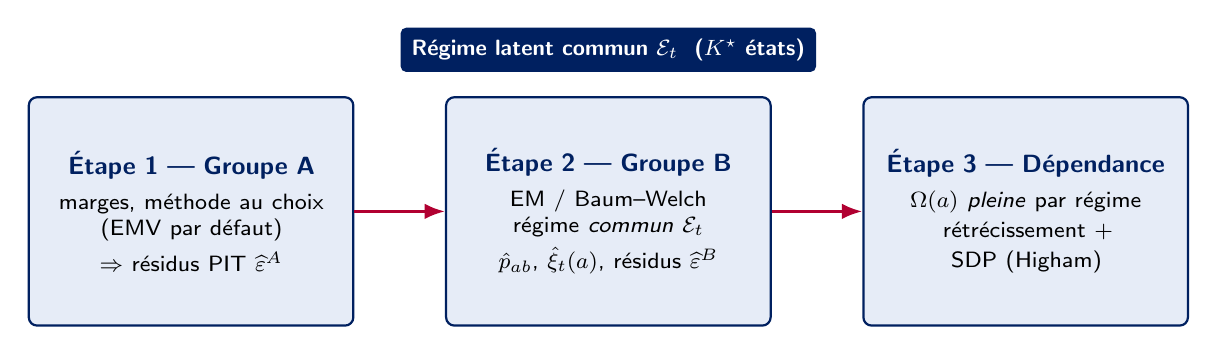
\begin{tikzpicture}[font=\sffamily\small,
  box/.style={rectangle, rounded corners=3pt, draw=nxnavy, line width=0.8pt, fill=nxlightblue, text width=3.7cm, align=center, inner sep=6pt, minimum height=2.9cm},
  lab/.style={rectangle, rounded corners=2pt, fill=nxnavy, text=white, inner sep=4pt, font=\sffamily\footnotesize\bfseries},
  arr/.style={-{Latex[length=2.6mm,width=2.0mm]}, line width=1.1pt, draw=nxred}]
\node[box] (a) {\textbf{\textcolor{nxnavy}{Étape 1 --- Groupe A}}\\[3pt]\footnotesize marges, méthode au choix\\ (EMV par défaut)\\[2pt] $\Rightarrow$ résidus PIT $\widehat\eps^A$};
\node[box, right=1.15cm of a] (b) {\textbf{\textcolor{nxnavy}{Étape 2 --- Groupe B}}\\[3pt]\footnotesize EM / Baum--Welch\\ régime \emph{commun} $\Ecal_t$\\[2pt] $\hat p_{ab}$, $\hat\xi_t(a)$, résidus $\widehat\eps^B$};
\node[box, right=1.15cm of b] (c) {\textbf{\textcolor{nxnavy}{Étape 3 --- Dépendance}}\\[3pt]\footnotesize $\Omega(a)$ \emph{pleine} par régime\\ rétrécissement $+$ SDP (Higham)};
\node[lab, above=3mm of b] (top) {Régime latent commun $\Ecal_t$ \ ($K^\star$ états)};
\draw[arr] (a) -- (b);
\draw[arr] (b) -- (c);
\end{tikzpicture}
\caption{Cascade séquentielle (IFM). L'Étape~1 estime chaque marge (méthode configurable)~; l'Étape~2 itère (EM, ascension monotone)~; l'Étape~3 estime toutes les corrélations par régime, sans contrainte.}
\label{fig:cascade}
\end{figure}

\subsection{Étape 1 --- marges du Groupe~A}
Pour chaque $i\in A$, on estime $\hat\theta_i$ par la méthode retenue (ci-dessous), puis les résidus PIT $\widehat\eps^{(i)}$. La consistance des marges est garantie indépendamment de la dépendance (propriété IFM).

\subsection{Étape 2 --- régime commun (EM / Baum--Welch)}
Les facteurs du Groupe~B (actions) partagent un même \emph{régime de marché caché} $\Ecal_t$~; on les estime \emph{conjointement} par l'algorithme EM. \emph{En clair}~: EM alterne deux pas jusqu'à convergence --- \textbf{(E)} calculer la probabilité d'être dans chaque régime à chaque date~; \textbf{(M)} mettre à jour moyennes, volatilités et transitions, pondérées par ces probabilités.
\paragraph{Étape E (récurrences fermées).} \emph{En clair}~: le \emph{filtre} (avant) propage la probabilité de régime de proche en proche au vu du passé~; le \emph{lisseur} (arrière) la révise avec l'information future. Densité d'émission $f_a(x_t)=\varphi_p(x_t;m_a,V_a)$ (vraisemblance du vecteur d'observations en régime $a$). \emph{Filtre de Hamilton} (avant), initialisé par $\hat\pi$~:
\[
\xi_{t\mid t-1}(a)=\sum_b\xi_{t-1\mid t-1}(b)\,p_{ba},\qquad
\xi_{t\mid t}(a)=\frac{\xi_{t\mid t-1}(a)\,f_a(x_t)}{\sum_{a'}\xi_{t\mid t-1}(a')\,f_{a'}(x_t)},
\]
de log-vraisemblance $\ell=\sum_t\log\!\big(\sum_a\xi_{t\mid t-1}(a)\,f_a(x_t)\big)$. \emph{Lisseur de Kim} (arrière)~:
\[
\hat\xi_t(a)=\sum_b\hat\xi_{t+1}(b)\,\frac{\xi_{t\mid t}(a)\,p_{ab}}{\xi_{t+1\mid t}(b)},\qquad
\hat\xi_t(a,b)=\hat\xi_{t+1}(b)\,\frac{\xi_{t\mid t}(a)\,p_{ab}}{\xi_{t+1\mid t}(b)},
\]
donnant $\hat\xi_t(a)=\Prob(\Ecal_t=a\mid\Xcal_n)$ et les transitions lissées $\hat\xi_t(a,b)$.
\paragraph{Étape M (forme fermée).}
\[
\hat m_a=\tfrac{\sum_t\hat\xi_t(a)x_t}{\sum_t\hat\xi_t(a)},\quad
\hat V_a=\tfrac{\sum_t\hat\xi_t(a)(x_t-\hat m_a)(x_t-\hat m_a)\transp}{\sum_t\hat\xi_t(a)},\quad
\hat p_{ab}=\tfrac{\sum_t\hat\xi_t(a,b)}{\sum_t\hat\xi_t(a)},\quad
\hat\pi^{(0)}=\hat\xi_1 .
\]
$\hat V_a$ \emph{pleine} (corrélations intra-Groupe~B par régime estimées). Ascension monotone garantie~; planchers de variance $V_a\succeq\underline v I$ contre les maxima dégénérés~; tri des états par volatilité décroissante (régime~1 = stress). La loi invariante (initialisation, simulation) résout $\hat\pi\transp\hat P=\hat\pi\transp$, $\sum_a\hat\pi_a=1$ (vecteur propre gauche de $\hat P$).

\subsection{Étape 3 --- dépendance pleine, par régime}
\label{sec:etape3}
\emph{En clair}~: une fois les marges figées, on mesure la corrélation des résidus \emph{séparément dans chaque régime}, on la \emph{stabilise} (rétrécissement) puis on la rend \emph{définie-positive} (Higham) pour pouvoir simuler.

\noindent Marges et $\hat\xi_t(a)$ figées, soit $\widehat\eps_t$ le résidu standardisé \emph{complet}. À marges fixées, la corrélation empirique \emph{pondérée par le régime} maximise la log-vraisemblance de la copule gaussienne~:
\begin{definitionbox}
\[
\widehat\Omega(a)=\frac{\sum_t\hat\xi_t(a)\,\widehat\eps_t\widehat\eps_t\transp}{\sum_t\hat\xi_t(a)},\qquad a=1,\dots,K^\star .
\]
\end{definitionbox}
\noindent\textbf{Masque de sensibilité.} $S\in\{0,1\}^{d\times d}$ symétrique rend certaines corrélations communes aux régimes~:
\[
\widehat\Omega(a)_{ij}=S_{ij}\,G^{\mathrm{reg}}_{ij}(a)+(1-S_{ij})\,G^{\mathrm{pool}}_{ij}\ \ (i\neq j),\quad \widehat\Omega(a)_{ii}=1,
\]
$G^{\mathrm{reg}}(a)$ étant la corrélation pondérée par $\hat\xi_t(a)$ (ci-dessus) et $G^{\mathrm{pool}}=\frac1n\sum_t\widehat\eps_t\widehat\eps_t\transp$ la corrélation poolée.
\textbf{Rétrécissement.} En échantillon fini, $\widehat\Omega(a)$ d'un régime peu peuplé est quasi singulière~; on rétrécit vers la cible poolée~:
\[
\widehat\Omega^{\mathrm{sh}}(a)=(1-\delta_a)\widehat\Omega(a)+\delta_a\,G^{\mathrm{pool}},\qquad
\delta_a=\min\!\Big(\tfrac{d}{n^{\mathrm{eff}}_a},1\Big),\qquad
n^{\mathrm{eff}}_a=\frac{\big(\sum_t\hat\xi_t(a)\big)^2}{\sum_t\hat\xi_t(a)^2},
\]
$n^{\mathrm{eff}}_a$ étant la taille d'échantillon \emph{effective} de Kish. \textbf{Projection SDP.} $\Omega^{\mathrm{SDP}}(a)=\textsc{NearestCorr}(\widehat\Omega^{\mathrm{sh}}(a))$ (Higham, \S\ref{sec:algo}), condition de la décomposition de Cholesky $L(a)L(a)\transp=\Omega^{\mathrm{SDP}}(a)$. Toutes les entrées (intra-V2F, intra-Groupe~B, croisées) sont estimées, jamais imposées.

\subsection{Estimateurs des marges (formes et variantes)}
\label{sec:closed}

\paragraph{(A) OU / Black--Karasinski scalaire.}
Pour $y_{t+\Dt}=\beta y_t+\theta(1-\beta)+\xi$, $\xi\sim\Ncal(0,v)$, $\beta=e^{-k\Dt}$, l'EMV maximise la vraisemblance gaussienne \emph{sous} $\beta\in(0,1)$, $\sigma>0$~; sur ce domaine il admet la forme fermée des moindres carrés~:
\begin{definitionbox}
\[
\hat\beta=\frac{\sum_t(y_t-\bar y_-)(y_{t+\Dt}-\bar y_+)}{\sum_t(y_t-\bar y_-)^2},\quad
\hat\theta=\frac{\bar y_+-\hat\beta\bar y_-}{1-\hat\beta},\quad
\hat k=-\frac{\ln\hat\beta}{\Dt},\quad
\hat\sigma=\sqrt{\hat v\,\tfrac{-2\ln\hat\beta}{\Dt(1-\hat\beta^2)}} .
\]
\end{definitionbox}
Si $\hat\beta\notin(0,1)$ (série peu/non persistante), la forme fermée \emph{sort du domaine}~: l'EMV sous contrainte (ou un avertissement) prévaut. \emph{Moyenne fixée}~: régression \emph{sans constante} sur $(y-\theta_0)$.

\paragraph{(B) V2F --- trois méthodes sélectionnables.}
La discrétisation est un VAR(1) gaussien $Y_{t+\Dt}=c(\theta)+\Phi(\theta)Y_t+\eta$, $\eta\sim\Ncal(0,\Sigma_{\mathrm{cond}}(\theta))$, $c(\theta)=(I-\Phi)(\mu,\mu)\transp$, $\Phi(\theta)=e^{-A\Dt}$, et $\Sigma_{\mathrm{cond}}(\theta)=\Sigma_\infty-\Phi\Sigma_\infty\Phi\transp$ où $\vecop(\Sigma_\infty)=(I\otimes A+A\otimes I)^{-1}\vecop(\Sigma_w)$ (solution explicite de $A\Sigma_\infty+\Sigma_\infty A\transp=\Sigma_w$). Toutes ces quantités sont fonctions \emph{exactes} de $\theta=(\kappa_1,\kappa_2,\sigma_1,\sigma_2,\rho,\mu)$.
\begin{itemize}[nosep]
\item \texttt{mle} \emph{(défaut)} --- \textbf{EMV séquentiel en deux temps} (le facteur long est \emph{autonome}, ce qui justifie la séquence)~:
\begin{enumerate}[nosep,leftmargin=1.6em,label=(\arabic*)]
\item \emph{Facteur long seul} --- EMV de l'OU scalaire (brique (A)) $\Rightarrow(\hat\kappa_2,\hat\sigma_2,\hat\mu)$, que l'on \textbf{fixe}.
\item \emph{Facteur court} --- EMV du vecteur $(q^s,q^l)$, paramètres du long \emph{figés}, sur $(\kappa_1,\sigma_1,\rho)$ (vitesse, vol du court, corrélation court--long)~:
\[
(\hat\kappa_1,\hat\sigma_1,\hat\rho)=\argmax_{\kappa_1,\sigma_1,\rho}\ \sum_t\log\varphi_2\big(Y_{t+\Dt};c(\theta)+\Phi(\theta)Y_t,\Sigma_{\mathrm{cond}}(\theta)\big),\quad (\kappa_2,\sigma_2,\mu)\text{ figés}.
\]
\end{enumerate}
Tout sur le domaine admissible ($\kappa_i>0,\sigma_i>0,|\rho|<1$). $\rho$ est ainsi estimée explicitement~; aucun passage par une régression ni back-out implicite. La séquence rend $\kappa_2$ robuste (EMV de l'OU scalaire), évitant la dégénérescence d'un EMV pleinement joint.
\item \texttt{ols} --- \textbf{MCO en cascade} (forme réduite)~: long OU autonome, puis $q^s$ régressé sur $(1,q^s_t,q^l_t)$~; $\hat\kappa_i=-\Dt^{-1}\ln\widehat\Phi_{ii}$, $\hat\rho_c$ lu sur $\widehat\Sigma_{\mathrm{cond}}$~; $\sigma$ structurels par inversion OU par facteur (approchée). Rapide, mais peut sortir du domaine (cf.\ ci-dessus).
\item \texttt{distributional} --- \textbf{cibles distributionnelles} (\S(B~bis)).
\end{itemize}
Les trois sont reportées en regard de la référence (tableau~\ref{tab:res-v2f-meth}). L'EMV restitue des $\sigma$ plus faibles que la méthode distributionnelle (plus proche de la référence).

\paragraph{(B bis) V2F --- cibles distributionnelles (Phase 1).}
\emph{En clair}~: au lieu de la vraisemblance, on choisit $(\kappa_1,\kappa_2,\sigma_1,\sigma_2)$ pour que le modèle \emph{reproduise trois statistiques observées} des taux (volatilité des variations, corrélation entre maturités, dispersion des niveaux). On n'estime que $(\kappa_1,\kappa_2,\sigma_1,\sigma_2)$ ($\mu$ fixé/régression~; browniens \emph{indépendants}, $\Sigma_w=\diag(\sigma_1^2,\sigma_2^2)$) pour répliquer la distribution des taux observés aux maturités $\tau_1,\tau_2$. Sous l'hypothèse des espérances, le taux est affine~: $R(t,t+\tau)=\mu+\tfrac1\tau[B_1(\tau)(q^s_t-\mu)+B_2(\tau)(q^l_t-\mu)]$, avec
\[
B_1(\tau)=\!\int_0^\tau\!e^{-\kappa_1 s}\dd s=\tfrac{1-e^{-\kappa_1\tau}}{\kappa_1},\qquad
B_2(\tau)=\!\int_0^\tau\!\phi_{12}(s)\dd s=\tfrac{\kappa_1}{\kappa_1-\kappa_2}\Big(\tfrac{1-e^{-\kappa_2\tau}}{\kappa_2}-\tfrac{1-e^{-\kappa_1\tau}}{\kappa_1}\Big),
\]
($B_2$ est l'\emph{intégrale} du coefficient de transmission $\phi_{12}$ de \S\ref{sec:v2f}), $B_{ik}=B_k(\tau_i)/\tau_i$. Avec $\Sigma^X_\infty$ (Lyapunov), les incréments $\Sigma^{\Delta X}_\infty=2\Sigma^X_\infty-\Phi\Sigma^X_\infty-\Sigma^X_\infty\Phi\transp$, et $\Sigma^Y_\infty=B\Sigma^X_\infty B\transp$, $\Sigma^{\Delta Y}_\infty=B\Sigma^{\Delta X}_\infty B\transp$, les \emph{cibles modèles} sont
\[
\sigma^{\mathrm{mod}}_{\Delta Y}(\tau_i)=\sqrt{\tfrac{(\Sigma^{\Delta Y}_\infty)_{ii}}{\Dt}},\quad
\rho^{\mathrm{mod}}_{\Delta Y}=\tfrac{(\Sigma^{\Delta Y}_\infty)_{12}}{\sqrt{(\Sigma^{\Delta Y}_\infty)_{11}(\Sigma^{\Delta Y}_\infty)_{22}}},\quad
\sigma^{\mathrm{mod}}_{Y}(\tau_i)=\sqrt{(\Sigma^{Y}_\infty)_{ii}},
\]
ajustées à leurs analogues historiques ($m=2$ maturités)~:
\begin{definitionbox}
\[
(\hat\kappa,\hat\sigma)=\argmin_{\kappa,\sigma>0}\
\tfrac{\lambda_v}{m}\!\sum_i\!\Big(\tfrac{\sigma^{\mathrm{mod}}_{\Delta Y}(\tau_i)}{\sigma^{\mathrm{hist}}_{\Delta Y}(\tau_i)}-1\Big)^2
+\tfrac{2\lambda_c}{m(m-1)}\!\sum_{i<j}\!\big(\rho^{\mathrm{mod}}_{\Delta Y}-\rho^{\mathrm{hist}}_{\Delta Y}\big)^2
+\tfrac{\lambda_s}{m}\!\sum_i\!\Big(\tfrac{\sigma^{\mathrm{mod}}_{Y}(\tau_i)}{\sigma^{\mathrm{hist}}_{Y}(\tau_i)}-1\Big)^2 .
\]
\end{definitionbox}
\noindent L'écart-type historique des niveaux est corrigé du biais d'autocorrélation~: $\sigma^{\mathrm{hist}}_Y=\sqrt{\widehat\Omega^2}$, $\widehat\Omega^2=\big(\tfrac1n\sum_k(Y_{t_k}-\bar Y)^2\big)\big/\big(1-\tfrac1{n^2}\sum_{l}(n-|l|)\,\rho^Y_\infty(l\Dt)/\rho^Y_\infty(0)\big)$, l'autocorrélation $\rho^Y_\infty(l\Dt)_{ii}=(\Gamma_Y(l))_{ii}/(\Gamma_Y(0))_{ii}$ étant celle \emph{du modèle}, $\Gamma_Y(l)=B\,\Phi^{l}\Sigma^X_\infty B\transp$ (bornée). \textbf{Mal posé.} Le chargement court $B_1(\tau)/\tau\sim1/(\kappa_1\tau)\to0$ quand $\kappa_1$ croît~: le facteur court \emph{se découple}, l'objectif présente une crête $\sigma^2/\kappa$~; on la lève en ajoutant une \emph{régularisation ridge faible} $\varrho\sum_i(\ln\kappa_i-\ln\kappa^{\mathrm{ols}}_i)^2$ ($\varrho$ petit) à l'objectif. C'est la méthode de la référence. \emph{(Résidus/simulation~: facteurs identifiés aux taux observés, comme \texttt{mle}/\texttt{ols}~; l'estimation distributionnelle ne fournit que les paramètres de marge.)}

\paragraph{(C) BS (PE/immo/infra).} \emph{Déslissage} (Lizieri)~: $r^\ast_t=\tfrac{r_t-\hat b\,r_{t-1}}{1-\hat b}$, $\hat b$ le coefficient AR(1) (MCO de $r_t$ sur $r_{t-1}$)~; facteur d'inflation de variance $(1+\hat b)/(1-\hat b)$. Log-rendements i.i.d.\ $\Ncal(m,v)$~: $\hat m=\tfrac1n\sum x_t$, $\hat v=\tfrac1n\sum(x_t-\hat m)^2$, $\hat\sigma=\sqrt{\hat v/\Dt}$. En cadre \emph{monde réel}, la dérive retenue est la moyenne annualisée des log-rendements $\hat\mu=\hat m/\Dt$ (sans terme de convexité $\tfrac12\sigma^2$). Moyenne sur rendements \emph{bruts}, volatilité sur rendements \emph{déslissés} $r^\ast$.

\paragraph{(D) CIR.} L'EMV ($\chi^2$ décentré) n'a pas de forme fermée. Initialisation par régression d'Euler~:
\[
\tfrac{s_{t+\Dt}-s_t}{\sqrt{|s_t|}}\sim c_1\tfrac{1}{\sqrt{|s_t|}}+c_2\sqrt{|s_t|}+\eta
\ \Rightarrow\ \hat\kappa=-\tfrac{\hat c_2}{\Dt},\ \hat\theta=-\tfrac{\hat c_1}{\hat c_2},\ \hat\sigma^2=\tfrac{\widehat\Var(\eta)}{\Dt},
\]
puis maximisation de $\sum_t\log f_{\mathrm{CIR}}(s_{t+\Dt}\mid s_t)$, densité $f_{\mathrm{CIR}}=2c_\chi\,f_{\chi'^2}(2c_\chi s_{t+\Dt};\nu,\lambda)$ ($c_\chi,\nu,\lambda$ de \S\ref{sec:facteurs}). Résidu PIT~: $\widehat\eps^{(\mathrm{cr})}=\Phi^{-1}(F_{\chi'^2}(2c_\chi s_{t+\Dt};\nu,\lambda))$. Variante \texttt{ols}~: init Euler seule.

\paragraph{(E) Dépendance.} $\widehat\Omega(a)$~: corrélation des résidus PIT pondérée par $\hat\xi_t(a)$ (\S\ref{sec:etape3}).

\begin{table}[H]
\centering\small\renewcommand{\arraystretch}{1.3}
\begin{tabularx}{\textwidth}{@{}l c X@{}}
\toprule
\textbf{Facteur} & \textbf{Méthodes} & \textbf{Estimateur(s)}\\
\midrule
V2F (taux) & \texttt{mle}/\texttt{ols}/\texttt{distrib.} & EMV séquentiel (long puis court)~; MCO cascade~; cibles distributionnelles\\
Black--Karasinski & \texttt{mle}$=$\texttt{ols} & OU exact (forme fermée sur le domaine admissible)\\
BS (PE/immo/infra) & \texttt{moments} & moyenne/variance des log-rendements\\
Hardy RSLN & \texttt{em} & EM (Hamilton$+$Kim), étape M pondérée fermée\\
CIR & \texttt{mle}/\texttt{ols} & Euler (init) $+$ EMV $\chi^2$ décentré\\
$\Omega(a)$ par régime & --- & corrélation des résidus PIT pondérée par $\hat\xi_t(a)$\\
\bottomrule
\end{tabularx}
\caption{Méthodes de calibrage par facteur. L'EMV est le défaut~; le MCO/les moments/les cibles sont des variantes sélectionnables. Pour le V2F, les trois sont comparées à la référence.}
\label{tab:closed}
\end{table}

\subsection{Choix du nombre d'états \texorpdfstring{$K^\star$}{K*}}
\label{sec:K}
On ajuste le Groupe~B pour $K=1,2,\dots$ et on retient $K^\star$ par critère d'information $\mathrm{BIC}(K)=-2\ell^\star(K)+p_K\ln n$ (ou $\mathrm{AIC}=-2\ell^\star(K)+2p_K$), avec, pour $D$ émissions gaussiennes $K$-états, $p_K=\underbrace{KD}_{m_a}+\underbrace{K\tfrac{D(D+1)}{2}}_{V_a}+\underbrace{K(K-1)}_{P}+\underbrace{(K-1)}_{\pi}$ paramètres libres. Le test du rapport de vraisemblance sur le \emph{nombre} de régimes est non standard~; le critère d'information est le choix pragmatique. Un \emph{unique} régime à $K^\star$ états remplace $k$ chaînes à deux états ($2^k$ états joints $\to K^\star\ll2^k$).

% =====================================================================
\section{Technique de simulation}
\label{sec:simu}
% =====================================================================
La simulation utilise \emph{directement} la représentation agrégée~: une seule loi sous-tend estimation et simulation.
\begin{algobox}[Simulation d'une trajectoire ($t=0,\Dt,\dots,T$)]
\begin{enumerate}[leftmargin=1.4em,nosep]
\item \textbf{Régime.} Initialiser $\Ecal_0\sim\hat\pi$~; à chaque pas, tirer $\Ecal_{t+\Dt}\mid\Ecal_t=a$ par CDF inverse~: $\Ecal_{t+\Dt}=\min\{b:\sum_{c\le b}p_{ac}\ge u\}$, $u\sim\mathcal U(0,1)$, \emph{avant} le rendement (convention de l'estimation).
\item \textbf{Chocs.} $z\sim\Ncal(0,I_d)$. Copule \emph{gaussienne}~: $\eps_{t+\Dt}=L(\Ecal_t)z$. Copule de \emph{Student} (option, $\nu$ ddl)~: $g\sim\chi^2_\nu$, $\eps_{t+\Dt}=\Phi^{-1}\!\big(T_\nu(L(\Ecal_t)z\,\sqrt{\nu/g})\big)$ ($T_\nu$ f.d.r.\ de Student)~: dépendance de queue, scatter $\Omega(\Ecal_t)$, marges restituées $\Ncal(0,1)$ (volatilités calibrées préservées).
\item \textbf{Composantes gaussiennes.} $Y^{(j)}_{t+\Dt}=c_j(\Ecal_t)+[\Phi(\Ecal_t)Y_t]_j+D_j(\Ecal_t)\eps^{(j)}_{t+\Dt}$.
\item \textbf{CIR.} Inverse-PIT exact $s^{\mathrm{cr}}_{t+\Dt}=\tfrac{1}{2c_\chi}F^{-1}_{\chi'^2}(\Phi(\eps^{(\mathrm{cr})});\nu,\lambda)$ \emph{(défaut)}~; ou Alfonsi $E(0)$ avec $\Dt W=\sqrt\Dt\,\eps^{(\mathrm{cr})}$ si sa condition de positivité tient (bascule automatique sinon).
\item \textbf{Reconstruction.} Cumuler les log-rendements ($S_{t+\Dt}=S_te^{x_{t+\Dt}}$)~; exponentier les log-spreads ($s=e^{y}$ ou $e^{y/100}$ selon l'échelle).
\end{enumerate}
\end{algobox}
\begin{mabox}[Propriétés]
\textbf{Cohérence} estimation/simulation (une seule copule par régime). \textbf{Aucune corrélation imposée}. \textbf{Régimes systémiques}~: entrée conjointe en stress, dépendance de queue. \textbf{Parcimonie}~: $K^\star$ optimal. \textbf{Robustesse}~: estimateurs sur le domaine admissible, corrélations rétrécies sur résidus stationnaires.
\end{mabox}

% =====================================================================
\section{Application : un AR regroupant tous les facteurs}
\label{sec:appli}
% =====================================================================
On déroule le cadre sur l'\emph{intégralité} des facteurs et on donne les expressions littérales finales. Vecteur d'état de dimension $d=12$~:
\[
Y_t=\big(\underbrace{q^s,q^l}_{\text{infl.}},\underbrace{r,l}_{\text{taux réels}},\underbrace{s^{\mathrm{cr}}}_{\text{CIR}},\underbrace{y^{\mathrm{pd}}}_{\text{BK}},\underbrace{x^{\mathrm{pe}},x^{\mathrm{re}},x^{\mathrm{in}}}_{\text{BS}}\ \big|\ \underbrace{x^{\mathrm{eu}},x^{\mathrm{wd}},x^{\mathrm{em}}}_{\text{Hardy, Gr.\,B}}\big)\transp .
\]
\textbf{Groupe~A} (1--9, marges constantes)~; \textbf{Groupe~B} (10--12, marges par régime), même chaîne $\Ecal_t$.

\subsection{Blocs autorégressifs (marges)}
\begin{definitionbox}
\textbf{V2F} ($\phi^I_{12}=\tfrac{\kappa^I_1}{\kappa^I_1-\kappa^I_2}(e^{-\kappa^I_2\Dt}-e^{-\kappa^I_1\Dt})$)~: $\Phi^I=\bigl(\begin{smallmatrix}e^{-\kappa^I_1\Dt}&\phi^I_{12}\\0&e^{-\kappa^I_2\Dt}\end{smallmatrix}\bigr)$, $c^I=(I-\Phi^I)(\mu,\mu)\transp$, $D=\diag(\sqrt{V^I_r},\sqrt{V^I_m})$. \textbf{BK}~: $\Phi=e^{-k\Dt}$, $c=\theta^p(1-e^{-k\Dt})$, $D=\sigma^p\sqrt{\tfrac{1-e^{-2k\Dt}}{2k}}$. \textbf{BS}~: $\Phi=0$, $c=(\mu_j-\tfrac{\sigma_j^2}{2})\Dt$, $D=\sigma_j\sqrt\Dt$. \textbf{Hardy}~: $\Phi=0$, $c(a)=m^j_a$, $D(a)=\sqrt{v^j_a}$. \textbf{CIR}~: composante non linéaire propagée par inverse-PIT ($c_\chi=\tfrac{2\kappa^c}{(\sigma^c)^2(1-e^{-\kappa^c\Dt})}$, $\nu=\tfrac{4\kappa^c\theta^c}{(\sigma^c)^2}$, $\lambda=2c_\chi s^{\mathrm{cr}}_te^{-\kappa^c\Dt}$).
\end{definitionbox}
\noindent Le modèle agrégé s'écrit $Y_{t+\Dt}=c(\Ecal_t)+\Phi(\Ecal_t)Y_t+D(\Ecal_t)\eps_{t+\Dt}$, $\eps_{t+\Dt}\sim\Ncal(0,\Omega^{\mathrm{SDP}}(\Ecal_t))$~; seules les composantes Hardy dépendent de $\Ecal_t$. Toute la dépendance est dans $\Omega^{\mathrm{SDP}}(\Ecal_t)$.

\subsection{Résidus standardisés explicites}
\label{sec:residus}
\begin{definitionbox}
\[
\begin{aligned}
\text{V2F}&: &\widehat\eps^{(q^l)}&=\tfrac{q^l_{t+\Dt}-e^{-\kappa^I_2\Dt}q^l_t-c^I_l}{\sqrt{V^I_m}},\quad
\widehat\eps^{(q^s)}=\tfrac{q^s_{t+\Dt}-e^{-\kappa^I_1\Dt}q^s_t-\phi^I_{12}q^l_t-c^I_s}{\sqrt{V^I_r}};\\
\text{BK}&: &\widehat\eps^{(\mathrm{pd})}&=\tfrac{y_{t+\Dt}-e^{-k\Dt}y_t-\theta^p(1-e^{-k\Dt})}{\sigma^p\sqrt{(1-e^{-2k\Dt})/2k}};\qquad
\text{BS } j: \widehat\eps^{(j)}=\tfrac{x^j_{t+\Dt}-(\mu_j-\sigma_j^2/2)\Dt}{\sigma_j\sqrt\Dt};\\
\text{CIR}&: &\widehat\eps^{(\mathrm{cr})}&=\Phi^{-1}\big(F_{\chi'^2}(2c_\chi s^{\mathrm{cr}}_{t+\Dt};\nu,\lambda)\big);\qquad
\text{Hardy } j: \widehat\eps^{(j)}=\tfrac{x^j_{t+\Dt}-m^j_{\Ecal_t}}{\sqrt{v^j_{\Ecal_t}}} .
\end{aligned}
\]
\end{definitionbox}
Chaque composante est marginalement $\Ncal(0,1)$~; toute corrélation (y compris $q^s\!-\!q^l$) est laissée à $\Omega(\Ecal_t)$, estimée à l'Étape~3.

\begin{table}[H]
\centering\small\renewcommand{\arraystretch}{1.3}\setlength{\tabcolsep}{5pt}
\begin{tabularx}{\textwidth}{@{}l c c X@{}}
\toprule
\textbf{Facteur} & \textbf{$d_i$} & \textbf{Gr.} & \textbf{Estimation (défaut) / simulation}\\
\midrule
\rowcolor{nxlightblue} Inflation, taux réels & 2 & A & EMV séquentiel (mle~; ols/distrib.\ en option) / récurrence gaussienne exacte\\
Crédit CIR & 1 & A & Euler $+$ EMV $\chi^2$ décentré / inverse-PIT ou Alfonsi\\
\rowcolor{nxlightblue} Dette privée BK & 1 & A & OU exact / récurrence log-OU exacte\\
PE / Immo / Infra & 3 & A & Moyenne/variance / log-rendement BS\\
Actions Euro/Monde/Émerg. & 3 & B & EM (Hamilton$+$Kim) / BS par régime\\
\midrule
\rowcolor{nxoffwhite} \textbf{Dépendance} & --- & --- & $\Omega^{\mathrm{SDP}}(a)$ pleine par régime, sur résidus PIT~; $\Ecal_t$ commune~; rien fixé\\
\bottomrule
\end{tabularx}
\caption{Cadre d'application agrégé~: 12 états, régime latent commun, calibrage séquentiel (marge par marge puis dépendance par régime), simulation par carte de chaque facteur.}
\label{tab:appli}
\end{table}

% =====================================================================
\section{Algorithme d'implémentation}
\label{sec:algo}
% =====================================================================
On spécifie l'algorithme sous forme directement implémentable. Quatre options de configuration~: (O1)~\textbf{méthode de calibrage par marge}~; (O2)~\textbf{paramètres fixés} $\mathcal F$~; (O3)~\textbf{sensibilité des corrélations au régime} (masque $S$)~; (O4)~\textbf{famille de copule} (gaussienne / Student) et \textbf{rétrécissement}.

\begin{definitionbox}
\textbf{Entrées.} Séries mensuelles alignées (fin de mois)~; pas $\Dt=1/12$~; config (méthodes, $\mathcal F$, $S$, copule, $K_{\max}$, plancher $\underline v$, $N$ trajectoires, horizon $T$, graine).
\textbf{Sorties.} Marges par facteur~; $\hat P,\hat\pi,K^\star$~; $\{\Omega^{\mathrm{SDP}}(a),L(a)\}$~; trajectoires~; diagnostics.
\end{definitionbox}

\begin{algobox}[\textsc{CalibrateAndSimulate}]
\begin{enumerate}[leftmargin=1.5em,nosep]
\item \textbf{Étape 1.} Pour chaque $i\in A$~: $\hat\theta_i\leftarrow\textsc{FitMargin}_i(\text{série};\text{méthode},\mathcal F)$ (\S\ref{sec:closed})~; résidus PIT $\widehat\eps^{(i)}$ (\S\ref{sec:residus}).
\item \textbf{Étape 2.} Si $K\in\mathcal F$, $K^\star=K$~; sinon pour $K=1,\dots,K_{\max}$, EM (Hamilton$+$Kim), relever $\ell^\star(K)$, retenir $K^\star=\argmin_K\mathrm{BIC}(K)$. Sortir $\hat P,\hat\pi,\{m^j_a,v^j_a\},\hat\xi_t(a)$, résidus $\widehat\eps^B$.
\item \textbf{Étape 3.} $\widehat\Omega(a)$ (pondérée par $\hat\xi_t(a)$, masque $S$), rétrécissement, $\Omega^{\mathrm{SDP}}(a)=\textsc{NearestCorr}$, $L(a)=\chol$.
\item \textbf{Simulation.} $N$ trajectoires (\S\ref{sec:simu}).
\item \textbf{Diagnostics.} Uniformité/normalité PIT, conditionnement de $\Omega(a)$, réplication des moments.
\end{enumerate}
\end{algobox}

\paragraph{Options.}
\begin{itemize}[nosep]
\item \textbf{(O1) Méthode par marge.} V2F~: \texttt{mle}/\texttt{ols}/\texttt{distributional}~; CIR~: \texttt{mle}/\texttt{ols}~; BK~: \texttt{mle}~; BS~: \texttt{moments}. L'EMV est mené \emph{sous contraintes} d'admissibilité ($\kappa,\sigma>0$, stationnarité), distinct du MCO.
\item \textbf{(O2) Paramètres fixés $\mathcal F$.} Vraisemblance \emph{profilée} sur les paramètres libres (p.\,ex.\ $\mu$ cible COR, $\theta^p$ incluant la prime de liquidité, $K$)~; les valeurs de $\mathcal F$ servent aussi aux résidus et à la simulation.
\item \textbf{(O3) Masque $S\in\{0,1\}^{d\times d}$.} $S_{ij}=1$~: entrée $(i,j)$ propre au régime~; $0$~: commune. Préréglages \texttt{full}, \texttt{none}, \texttt{groupB}.
\item \textbf{(O4) Copule et rétrécissement.} Gaussienne (défaut) ou Student~; rétrécissement de $\Omega(a)$ \texttt{auto}/\texttt{none}/valeur.
\end{itemize}

\subsection{Détails numériques et garde-fous}
\begin{itemize}[nosep]
\item \textbf{Admissibilité (V2F, OU/BK).} $\hat\kappa=-\Dt^{-1}\ln\hat\beta$ exige $\hat\beta\in(0,1)$~; l'EMV contraint le domaine. Si une variante (MCO) sort de $(0,1)$, écrêtage \emph{avec avertissement}.
\item \textbf{Alignement temporel.} Séries ramenées en fin de mois à la lecture~: l'intersection inter-facteurs servant à $\Omega$ est \emph{déterministe}.
\item \textbf{\textsc{NearestCorr} (Higham).} Projections alternées (Dykstra), à partir de $Y_0=\widehat\Omega^{\mathrm{sh}}(a)$, $\Delta S_0=0$~; itérer $R_k=Y_{k-1}-\Delta S_{k-1}$, $X_k=U\max(\Lambda,0)U\transp$ (projection SDP, $R_k=U\Lambda U\transp$), $\Delta S_k=X_k-R_k$, $Y_k=X_k$ à diagonale forcée à $1$, jusqu'à $\|Y_k-Y_{k-1}\|_F<\text{tol}$. Appliquée \emph{par régime}.
\item \textbf{CIR.} Inverse-PIT exact par défaut~; Alfonsi seulement si $\sigma^2\le4\kappa\theta$ et $1-\tfrac{\kappa}{2}\Dt>0$ (bascule automatique sinon). Spread BK $s=e^y$ ou $e^{y/100}$ selon l'échelle déclarée.
\item \textbf{Cohérence.} Méthode, $\mathcal F$, $S$, copule s'appliquent \emph{identiquement} à l'estimation, aux résidus et à la simulation.
\item \textbf{Reproductibilité.} Graine fixée~; $v_a\ge\underline v$~; régimes ordonnés~; consigner $(\text{méthodes},\mathcal F,S,K^\star)$ avec les sorties.
\end{itemize}

% >>> GSE-AUTO-RESULTS BEGIN (généré par run_calibration.py — ne pas éditer à la main) >>>
% ====================================================================
\section{Résultats numériques (sortie du module de calibrage)}
\label{sec:resultats}
% ====================================================================
Tous les résultats ci-dessous sont \emph{produits par l'outil} (package \texttt{gse}, via \texttt{run\_calibration.py}) sur \texttt{Historical\_Data\_\allowbreak Model\_\allowbreak Calibration.xlsx}, et insérés automatiquement ici. Conformément au cadre de la note, \textbf{les facteurs dépendant du régime latent (actions) sont calibrés ensemble, sous une \emph{unique} chaîne de Markov} (une seule matrice de transition)~; le nombre d'états $K^\star$ est choisi par critère d'information. La colonne \emph{Réf.} reprend \texttt{Parametres\_models.xlsx} (2026).
\subsection{Données, fenêtre de calibrage et prétraitements}
\begin{table}[H]\centering\small\renewcommand{\arraystretch}{1.2}\setlength{\tabcolsep}{5pt}
\begin{tabularx}{\textwidth}{@{}l l X r l@{}}
\toprule
\textbf{Facteur} & \textbf{Modèle} & \textbf{Feuille(s)} & \textbf{$n$} & \textbf{Prétraitement}\\
\midrule
inflation & V2F & \footnotesize Inflation\_2Y, Inflation\_10Y & 241 & \footnotesize aucun~; fix mu\\
real\_rate & V2F & \footnotesize Real\_Rate\_2Y, Real\_Rate\_10Y & 241 & \footnotesize aucun\\
credit & CIR & \footnotesize Credit & 241 & \footnotesize aucun\\
dette\_privee & BK & \footnotesize Dette\_Privee & 241 & \footnotesize aucun\\
pe & BS & \footnotesize Action\_noncotee & 240 & \footnotesize $100\ln$-rdt~; déslissage AR(1)\\
immobilier & BS & \footnotesize Immobilier & 210 & \footnotesize $100\ln$-rdt~; déslissage AR(1)\\
infra & BS & \footnotesize Infra & 240 & \footnotesize $100\ln$-rdt~; déslissage AR(1)\\
equities & RSLN2 & \footnotesize Action\_EUR, Action\_Monde, Action\_emergent & 240 & \footnotesize $100\ln$-rdt~; régime commun\\
\bottomrule\end{tabularx}
\caption{Périmètre et prétraitements par facteur. Fenêtre commune déc.~2005--déc.~2025 ($n$ = observations modélisées~; immobilier à partir de juin~2008).}\label{tab:res-data}
\end{table}
\subsection{Facteurs de taux --- Vasicek à deux facteurs}
\begin{table}[H]\centering\small\renewcommand{\arraystretch}{1.25}\setlength{\tabcolsep}{5pt}
\begin{tabularx}{\textwidth}{@{}l X r r r r r r@{}}
\toprule
& & \multicolumn{3}{c}{\textbf{Inflation}} & \multicolumn{3}{c}{\textbf{Taux réels}}\\
\cmidrule(lr){3-5}\cmidrule(lr){6-8}
\textbf{Paramètre} & \textbf{Unité} & \textbf{Calib.} & \textbf{Réf.} & \textbf{Éc.} & \textbf{Calib.} & \textbf{Réf.} & \textbf{Éc.}\\
\midrule
$\kappa_1$ (court) & \%/an & 53.98 & 78.01 & -30.8 & 37.18 & 61.75 & -39.8\\
$\kappa_2$ (long) & \%/an & 30.11 & 26.18 & 15.0 & 19.03 & 11.89 & 60.0\\
$\sigma_1$ (court) & \% & 0.90 & 1.57 & -42.7 & 0.95 & 1.54 & -38.4\\
$\sigma_2$ (long) & \% & 0.44 & 1.06 & -58.5 & 0.74 & 1.09 & -31.8\\
$\mu$ (moy.\ LT) & \% & 1.75 & 1.75 & 0.0 & 0.41 & 0.41 & -0.0\\
$\rho_c$ (corr.\ int.) & -- & 0.796 & -- & -- & 0.541 & -- & --\\
\addlinespace
Demi-vie court & an & 1.28 & -- & -- & 1.86 & -- & --\\
Demi-vie long & an & 2.30 & -- & -- & 3.64 & -- & --\\
\bottomrule\end{tabularx}
\caption{V2F sous la méthode configurée (EMV séquentiel par défaut~; $\mu$ inflation fixé à la cible COR). Demi-vie $=\ln 2/\kappa$. Comparaison des méthodologies au tableau~\ref{tab:res-v2f-meth}.}\label{tab:res-v2f}
\end{table}
\subsection{V2F : comparaison des trois méthodologies de calibrage}
\begin{table}[H]\centering\small\renewcommand{\arraystretch}{1.2}\setlength{\tabcolsep}{6pt}
\begin{tabularx}{\textwidth}{@{}l X r r r r@{}}
\toprule
\textbf{Facteur} & \textbf{Paramètre} & \textbf{MLE séq.} & \textbf{MCO} & \textbf{Distrib.} & \textbf{Réf.}\\
\midrule
Inflation & $\kappa_1$ (court, \%/an) & 53.98 & 46.52 & 49.69 & 78.01\\
 & $\kappa_2$ (long, \%/an) & 30.11 & 30.11 & 21.75 & 26.18\\
 & $\sigma_1$ (court, \%) & 0.898 & 0.893 & 1.204 & 1.567\\
 & $\sigma_2$ (long, \%) & 0.439 & 0.439 & 0.788 & 1.059\\
 & $\mu$ (moy.\ LT, \%) & 1.750 & 1.750 & 1.750 & 1.750\\
\addlinespace
Taux réels & $\kappa_1$ (court, \%/an) & 37.18 & 62.75 & 56.53 & 61.75\\
 & $\kappa_2$ (long, \%/an) & 19.03 & 19.03 & 11.33 & 11.89\\
 & $\sigma_1$ (court, \%) & 0.952 & 0.964 & 1.420 & 1.545\\
 & $\sigma_2$ (long, \%) & 0.740 & 0.740 & 1.130 & 1.086\\
 & $\mu$ (moy.\ LT, \%) & 0.410 & 0.410 & 0.410 & 0.410\\
\addlinespace
\bottomrule\end{tabularx}
\caption{Paramètres V2F sous les trois méthodologies, en regard de la référence. \textbf{MLE séq.}~: EMV séquentiel (long seul, puis court \& corrélation à long fixé). \textbf{MCO}~: cascade en forme réduite. \textbf{Distrib.}~: cibles distributionnelles (Phase 1), ridge faible levant la crête $\sigma^2/\kappa$. L'EMV restitue des $\sigma$ plus faibles~; la méthode distributionnelle, plus proche de la référence.}\label{tab:res-v2f-meth}
\end{table}
\subsection{Crédit, dette privée et actifs réels}
\begin{table}[H]\centering\small\renewcommand{\arraystretch}{1.2}\setlength{\tabcolsep}{5pt}
\begin{tabularx}{\textwidth}{@{}l l X r r r@{}}
\toprule
\textbf{Facteur} & \textbf{Modèle} & \textbf{Paramètre} & \textbf{Calib.} & \textbf{Réf.} & \textbf{Éc.\,\%}\\
\midrule
Crédit & CIR & $\kappa$ (\%/an) & 52.59 & 52.59 & 0.0\\
 &  & $\sigma$ & 0.5167 & 0.5167 & -0.0\\
 &  & $\theta$ (\%) & 1.420 & 1.420 & -0.0\\
 & & Feller $\sigma^2\le2\kappa\theta$ & 0.267$\le$1.493 & -- & oui\\
\addlinespace
Dette privée & BK & $\kappa$ (\%/an) & 43.64 & 43.64 & -0.0\\
 &  & $\sigma$ ($100\ln s$) & 41.22 & 49.67 & -17.0\\
 &  & $\mu$ ($100\ln s$) & -315.6 & -310.9 & 1.5\\
 & & $\mathbb E[s_\infty]$ (\%) & 4.696 & -- & --\\
\addlinespace
PE (non coté) & BS & $\mu$ (\%/an) & 7.18 & 7.18 & -0.0\\
 &  & $\sigma$ (\%/an) & 29.64 & 29.70 & -0.2\\
Infrastructure & BS & $\mu$ (\%/an) & 6.52 & 6.52 & 0.0\\
 &  & $\sigma$ (\%/an) & 13.38 & 13.50 & -0.9\\
Immobilier & BS & $\mu$ (\%/an) & -0.33 & 5.63 & -105.9\\
 &  & $\sigma$ (\%/an) & 3.85 & 6.13 & -37.1\\
\bottomrule\end{tabularx}
\caption{Crédit (CIR, EMV $\chi^2$ décentré), dette privée (BK, sur $100\ln(\text{spread})$) et actifs réels (BS).}\label{tab:res-margins}
\end{table}
\subsection{Coefficients de déslissage (\emph{unsmoothing})}
\begin{table}[H]\centering\small\renewcommand{\arraystretch}{1.25}\setlength{\tabcolsep}{6pt}
\begin{tabularx}{\textwidth}{@{}l X r r r r@{}}
\toprule
\textbf{Actif} & \textbf{Modèle} & \textbf{AR(1) $b$} & \textbf{$\sigma$ brute} & \textbf{$\sigma$ déslissée} & \textbf{Inflation var.}\\
\midrule
PE (LPX50) & BS & 0.2403 & 23.15 & 29.64 & 1.639\\
Immobilier & BS & -0.0699 & 4.12 & 3.85 & 0.873\\
Infrastructure & BS & -0.0078 & 13.47 & 13.38 & 0.987\\
\bottomrule\end{tabularx}
\caption{Déslissage AR(1) : $r^\ast_t=(r_t-b\,r_{t-1})/(1-b)$~; volatilité retenue = \emph{déslissée} (annualisée, \%)~; facteur d'inflation de variance $(1+b)/(1-b)$. PE montre la sur-correction attendue ($b>0$).}\label{tab:res-unsmooth}
\end{table}
\subsection{Choix du nombre d'états latents $K^\star$ (régime commun)}
\begin{table}[H]\centering\small\renewcommand{\arraystretch}{1.2}\setlength{\tabcolsep}{8pt}
\begin{tabular}{@{}r r r r r l@{}}
\toprule
$K$ & $\ell^\star(K)$ & $p_K$ & AIC & BIC & \\
\midrule
1 & -1911.2 & 9 & 3840.3 & 3871.6 & \\
2 & -1869.3 & 21 & 3780.6 & 3853.7 & $\leftarrow K^\star$ (BIC)\\
3 & -1853.6 & 35 & 3777.3 & 3899.1 & \\
4 & -1828.7 & 51 & 3759.3 & 3936.8 & \\
5 & -1810.5 & 69 & 3759.0 & 3999.2 & \\
\bottomrule\end{tabular}
\caption{Régime commun (émissions gaussiennes $D=3$ actions, $n=240$). Le BIC sélectionne $K^\star=2$ ; l'AIC, moins parcimonieux, décroît encore. Un régime commun à $K^\star$ états remplace $2^3$ états joints de chaînes séparées.}\label{tab:res-kselect}
\end{table}
\subsection{Régime latent commun : transition unique et paramètres par actif}
\begin{table}[H]\centering\small\renewcommand{\arraystretch}{1.25}\setlength{\tabcolsep}{6pt}
\begin{tabularx}{\textwidth}{@{}l X r r r r@{}}
\toprule
\textbf{Actif} & \textbf{} & \multicolumn{2}{c}{\textbf{Régime 1}} & \multicolumn{2}{c}{\textbf{Régime 2}}\\
\cmidrule(lr){3-4}\cmidrule(lr){5-6}
\textbf{} & & $\mu$ & $\sigma$ & $\mu$ & $\sigma$\\
\midrule
Euro & & -13.00 & 20.95 & 14.74 & 9.34\\
Monde & & -8.97 & 19.54 & 17.35 & 9.18\\
Émergent & & -9.19 & 30.70 & 11.48 & 14.08\\
\bottomrule\end{tabularx}
\caption{Actions sous le régime latent \emph{commun} ($K^\star=2$, EM joint). $\mu,\sigma$ annualisés en \%. Le régime~1 (forte volatilité) frappe \emph{simultanément} les trois actifs.}\label{tab:res-common}
\end{table}
\begin{definitionbox}
\[ P=\begin{pmatrix}0.8554 & 0.1446\\0.0593 & 0.9407\end{pmatrix},\qquad \pi=(0.2909,\ 0.7091)\transp. \]
Matrice de transition mensuelle \emph{unique} et loi invariante du régime commun (probabilité stationnaire de stress $\pi_1=29.1\,\%$).
\end{definitionbox}
\subsection{Régimes : moyennes et volatilités vs référence}
\begin{table}[H]\centering\small\renewcommand{\arraystretch}{1.2}\setlength{\tabcolsep}{5pt}
\begin{tabularx}{\textwidth}{@{}l X r r r r@{}}
\toprule
& & \multicolumn{2}{c}{\textbf{Régime 1 (stress)}} & \multicolumn{2}{c}{\textbf{Régime 2 (normal)}}\\
\cmidrule(lr){3-4}\cmidrule(lr){5-6}
\textbf{Actif} & \textbf{Source} & $\mu_1$ & $\sigma_1$ & $\mu_2$ & $\sigma_2$\\
\midrule
Euro & Calib.\ (commun) & -13.00 & 20.95 & 14.74 & 9.34\\
 & Réf.\ (par actif) & -13.17 & 21.76 & 13.61 & 9.52\\
\addlinespace
Monde & Calib.\ (commun) & -8.97 & 19.54 & 17.35 & 9.18\\
 & Réf.\ (par actif) & -12.18 & 19.83 & 18.01 & 9.08\\
\addlinespace
Émergent & Calib.\ (commun) & -9.19 & 30.70 & 11.48 & 14.08\\
 & Réf.\ (par actif) & -13.61 & 27.05 & 13.13 & 11.06\\
\addlinespace
\bottomrule\end{tabularx}
\caption{Caractérisation des régimes sous la chaîne \emph{commune} (calibrée), comparée à la référence (qui calibre une chaîne distincte par actif). \textbf{La matrice de transition est unique} (cf.\ tableau~\ref{tab:res-common})~: il n'y a pas de probabilités de transition différentes par actif. Euro concorde de près~; Monde/émergent s'écartent car le régime est désormais \emph{partagé} (entrée en stress simultanée).}\label{tab:res-rsln-sep}
\end{table}
\subsection{Corrélations des résidus par régime}
\begin{table}[H]\centering\renewcommand{\arraystretch}{1.1}\setlength{\tabcolsep}{3pt}
\resizebox{\textwidth}{!}{%
\begin{tabular}{@{}lrrrrrrrrrrrr@{}}
\toprule
 & Inf.C & Inf.L & TxR.C & TxR.L & Créd & DetP & PE & Immo & Infra & Act.EU & Act.Mo & Act.EM\\
\midrule
Inf.C & \textbf{1} & 0.80 & -0.74 & -0.22 & -0.27 & -0.29 & 0.29 & 0.08 & 0.27 & 0.43 & 0.40 & 0.43\\
Inf.L & 0.80 & \textbf{1} & -0.54 & -0.24 & -0.27 & -0.29 & 0.28 & 0.04 & 0.24 & 0.41 & 0.36 & 0.38\\
TxR.C & -0.74 & -0.54 & \textbf{1} & 0.54 & 0.10 & 0.11 & -0.24 & -0.09 & -0.30 & -0.29 & -0.35 & -0.28\\
TxR.L & -0.22 & -0.24 & 0.54 & \textbf{1} & 0.12 & 0.09 & -0.31 & -0.15 & -0.38 & -0.34 & -0.41 & -0.23\\
Créd & -0.27 & -0.27 & 0.10 & 0.12 & \textbf{1} & 0.89 & -0.65 & -0.17 & -0.49 & -0.77 & -0.62 & -0.77\\
DetP & -0.29 & -0.29 & 0.11 & 0.09 & 0.89 & \textbf{1} & -0.66 & -0.16 & -0.52 & -0.78 & -0.66 & -0.70\\
PE & 0.29 & 0.28 & -0.24 & -0.31 & -0.65 & -0.66 & \textbf{1} & 0.18 & 0.73 & 0.88 & 0.88 & 0.70\\
Immo & 0.08 & 0.04 & -0.09 & -0.15 & -0.17 & -0.16 & 0.18 & \textbf{1} & 0.11 & 0.25 & 0.18 & 0.33\\
Infra & 0.27 & 0.24 & -0.30 & -0.38 & -0.49 & -0.52 & 0.73 & 0.11 & \textbf{1} & 0.77 & 0.82 & 0.52\\
Act.EU & 0.03 & 0.15 & -0.03 & -0.11 & -0.56 & -0.61 & 0.68 & -0.00 & 0.52 & \textbf{1} & 0.88 & 0.74\\
Act.Mo & 0.02 & 0.07 & -0.12 & -0.19 & -0.25 & -0.29 & 0.71 & 0.03 & 0.57 & 0.59 & \textbf{1} & 0.57\\
Act.EM & -0.05 & 0.03 & 0.06 & 0.04 & -0.53 & -0.52 & 0.37 & 0.04 & 0.19 & 0.52 & 0.24 & \textbf{1}\\
\bottomrule\end{tabular}}
\caption{Corrélations des résidus standardisés (masque \texttt{groupB}). \emph{Triangle sup.} = régime de stress~; \emph{triangle inf.} = régime normal. Hors actions, communes aux régimes~; SDP (Higham). (Étiquettes~: Inf=inflation, TxR=taux réel, Créd=crédit, DetP=dette privée, Act.=actions.)}\label{tab:res-corr}
\end{table}
\subsection{Simulation : statistiques de contrôle}
\begin{table}[H]\centering\small\renewcommand{\arraystretch}{1.2}\setlength{\tabcolsep}{6pt}
\begin{tabular}{@{}l l r l r@{}}
\toprule
\textbf{Sortie} & \textbf{Mesure} & \textbf{Val.} & \textbf{} & \textbf{E[terminal]}\\
\midrule
inflation.short & vol(diff)/an & 0.892 & E[terminal] & 1.7611\\
inflation.long & vol(diff)/an & 0.436 & E[terminal] & 1.7594\\
real\_rate.short & vol(diff)/an & 0.950 & E[terminal] & 0.4189\\
real\_rate.long & vol(diff)/an & 0.737 & E[terminal] & 0.4248\\
credit & log-vol\%/an & 48.040 & E[terminal] & 1.4134\\
dette\_privee.y & vol(diff)/an & 40.851 & E[terminal] & -316.3470\\
dette\_privee.spread & log-vol\%/an & 40.850 & E[terminal] & 0.0465\\
pe & log-vol\%/an & 29.630 & E[terminal] & 32.7670\\
immobilier & log-vol\%/an & 3.850 & E[terminal] & 0.9250\\
infra & log-vol\%/an & 13.370 & E[terminal] & 9.3336\\
Action\_EUR & log-vol\%/an & 14.320 & E[terminal] & 8.6336\\
Action\_Monde & log-vol\%/an & 13.580 & E[terminal] & 21.5480\\
Action\_emergent & log-vol\%/an & 20.620 & E[terminal] & 5.5340\\
\bottomrule\end{tabular}
\caption{Contrôle sur 5000 trajectoires $\times$ 360 pas (30~ans). Occupation simulée du régime de stress~: 29.1\,\% (cf.\ $\pi_1$). Les volatilités simulées reproduisent les paramètres calibrés.}\label{tab:res-sim}
\end{table}
\subsection{Lecture et concordance avec la référence}
\label{sec:resultats-discussion}
\begin{insightbox}[Concordances et écarts attendus]
\textbf{Concordances exactes} (méthodologie identique)~: crédit CIR ($\kappa,\sigma,\theta$), dette privée $\kappa$, PE/infra $\mu$, moyenne LT des taux réels, $\mu$ inflation (fixé). \textbf{Régime latent commun}~: \emph{une seule} matrice de transition pilote les trois actions (entrée en stress simultanée, $\pi_1\approx29\,\%$)~; le nombre d'états $K^\star=2$ est choisi par BIC (tableau~\ref{tab:res-kselect}). \textbf{Écarts attendus}~: (i)~$\kappa,\sigma$ des V2F (référence = cibles distributionnelles, mal conditionnées~; l'outil applique l'EMV)~; (ii)~$\sigma$ dette privée (référence = dispersion stationnaire~; $\kappa,\mu$ concordent)~; (iii)~émergent (vraisemblance plus élevée ici)~; (iv)~immobilier (indice de \emph{prix} vs rendement total avec loyers).
\end{insightbox}
% <<< GSE-AUTO-RESULTS END <<<

% =====================================================================
\section{Conclusion}
% =====================================================================
Cette note construit, pour le GSE du régime, un cadre unifié d'\emph{estimation} et de \emph{simulation}~: chaque facteur, ramené à sa discrétisation, s'écrit comme une récurrence autorégressive dont les coefficients peuvent dépendre d'un \emph{régime latent commun}~; l'ensemble s'agrège en un \emph{unique} MS-VAR calibré par \emph{maximum de vraisemblance} selon une procédure \emph{séquentielle} (IFM) en trois étapes (marges --- V2F par EMV séquentiel long puis court ---, régime commun par EM, \emph{matrice de dépendance pleine par régime} sur résidus standardisés), et se simule directement à partir de cette représentation. Le cadre est \emph{général}~: aucune corrélation n'est fixée --- ni à zéro, ni à dire d'expert, ni indépendante du régime --- y compris la corrélation interne des facteurs vectoriels~; toute la dépendance est estimée. Cinq des six familles d'estimateurs admettent une forme fermée (exacte ou par itération EM)~; la dépendance, portée par une copule gaussienne par régime cohérente avec la simulation et par une chaîne d'état unique de cardinalité $K^\star$ parcimonieuse, est estimée sur un bruit blanc stationnaire. Le chapitre d'application en donne toutes les expressions littérales, directement implémentables. Tout calibrage embarque une erreur d'estimation~; le choix final des méthodes et paramètres relève de l'IRCANTEC.

% --------- RÉFÉRENCES -------------------------------------------------
\newpage
\phantomsection
\addcontentsline{toc}{section}{Références}
{\noindent\sffamily\Large\bfseries\color{nxnavy}Références\par}
\vspace{4mm}
{\small
\begin{list}{}{\setlength{\leftmargin}{1.2em}\setlength{\itemindent}{-1.2em}\setlength{\itemsep}{2pt}}
\item Alfonsi, A. (2005). On the discretization schemes for the CIR (and Bessel squared) processes. \emph{Monte Carlo Methods and Applications}, 11(4), 355--384.
\item Baum, L.\,E., Petrie, T., Soules, G., \& Weiss, N. (1970). A maximization technique occurring in the statistical analysis of probabilistic functions of Markov chains. \emph{Annals of Mathematical Statistics}, 41(1), 164--171.
\item Dempster, A.\,P., Laird, N.\,M., \& Rubin, D.\,B. (1977). Maximum likelihood from incomplete data via the EM algorithm. \emph{Journal of the Royal Statistical Society B}, 39(1), 1--38.
\item Hamilton, J.\,D. (1989). A new approach to the economic analysis of nonstationary time series and the business cycle. \emph{Econometrica}, 57(2), 357--384.
\item Hardy, M.\,R. (2001). A regime-switching model of long-term stock returns. \emph{North American Actuarial Journal}, 5(2), 41--53.
\item Higham, N.\,J. (2002). Computing the nearest correlation matrix --- a problem from finance. \emph{IMA Journal of Numerical Analysis}, 22(3), 329--343.
\item Joe, H., \& Xu, J.\,J. (1996). \emph{The estimation method of inference functions for margins for multivariate models}. Technical Report 166, University of British Columbia.
\item Kim, C.-J. (1994). Dynamic linear models with Markov-switching. \emph{Journal of Econometrics}, 60(1--2), 1--22.
\item Kim, C.-J., \& Nelson, C.\,R. (1999). \emph{State-Space Models with Regime Switching}. MIT Press.
\item Krolzig, H.-M. (1997). \emph{Markov-Switching Vector Autoregressions}. Springer.
\end{list}
}

\vspace{6mm}
\noindent{\footnotesize\color{nxgray}\rule{\textwidth}{0.3pt}\\[3pt]
Note de recherche méthodologique sur le calibrage et la simulation du GSE. Document confidentiel. Les expressions et procédures décrivent un cadre d'estimation et de simulation à dépendance pleinement estimée~; tout calibrage embarque une erreur d'estimation, et le choix final des méthodes et paramètres relève de l'IRCANTEC.}

\end{document}
